\section{Theta Sketches}
\label{sec:theta}

Our first example is a $\Theta$ sketch implemented using  the 
\emph{K Minimum Values  (KMV)} algorithm~\cite{KMV}, 
which estimates the number of unique items in a data stream. 
A $\Theta$ sketch consisting of  $K$ samples provides an unbiased approximation $\hat{u}$ of the 
number $u$ of unique elements in the stream with a \emph{Relative Standard Error (RSE)} of $1/\sqrt{K-1}$.

%We first overview the sequential  sketch in Section~\ref{ssec:theta-overview}, 
%and then explain how we parallelize it in Section~\ref{ssec:concurrent-theta}.

\subsection{Overview}
\label{ssec:theta-overview}


A $\Theta$ sketch maintains a set of samples and a parameter $\Theta$
that determines which elements are added to the sample set (see Figure~\ref{fig:thetaSampling}). 
It uses a random hash function whose outputs are uniformly distributed
in the range $[0,1]$, and $\Theta$ is always in the same range.  
Every incoming data stream element is first hashed, and then the hash is compared to $\Theta$. 
In case it is smaller, the value is added to the sample set.  Otherwise, it is ignored. 

Because the hash outputs are uniformly distributed, an expected
portion $\Theta$ of them are smaller than $\Theta$ and hence included in the sample. 
Therefore, we can estimate the number of unique data items in the stream by
simply dividing the number of (unique) stored samples by $\Theta$.
The error depends on the size of the sample set -- $K$. 

 $\Theta$ sketches keep constant-size sample sets, independently of the stream size. 
 To this end, they need to adjust $\Theta$ on-the-fly, and prune elements of 
 the sample set whose hashes are greater than the new $\Theta$.
%There are a number of approaches to do that. 
The KMV solution keeps a sample of size $K$ 
holding the  values with the $K$ smallest hashes seen so far. 
In this case $\Theta$ is $1$ during the first $K$ updates, and 
subsequently it is the hash of the largest sample in the set.
Once the sample set is full,
every update that inserts  a new element also removes the largest
element in the set and updates $\Theta$ accordingly. 
%This can be implemented efficiently by keeping the samples in  a min-heap. 
%A nice property of this KMV variant is that it is \emph{order agnostic}, i.e., produces 
%identical results for streams that consist of the same elements albeit in a different order.
Note that since typically, $K \ll n$, the vast majority of hashes are larger than 
$\Theta$,  and so most update operations complete without updating the sample set. 


\begin{figure}[tb]
 %   \centering
    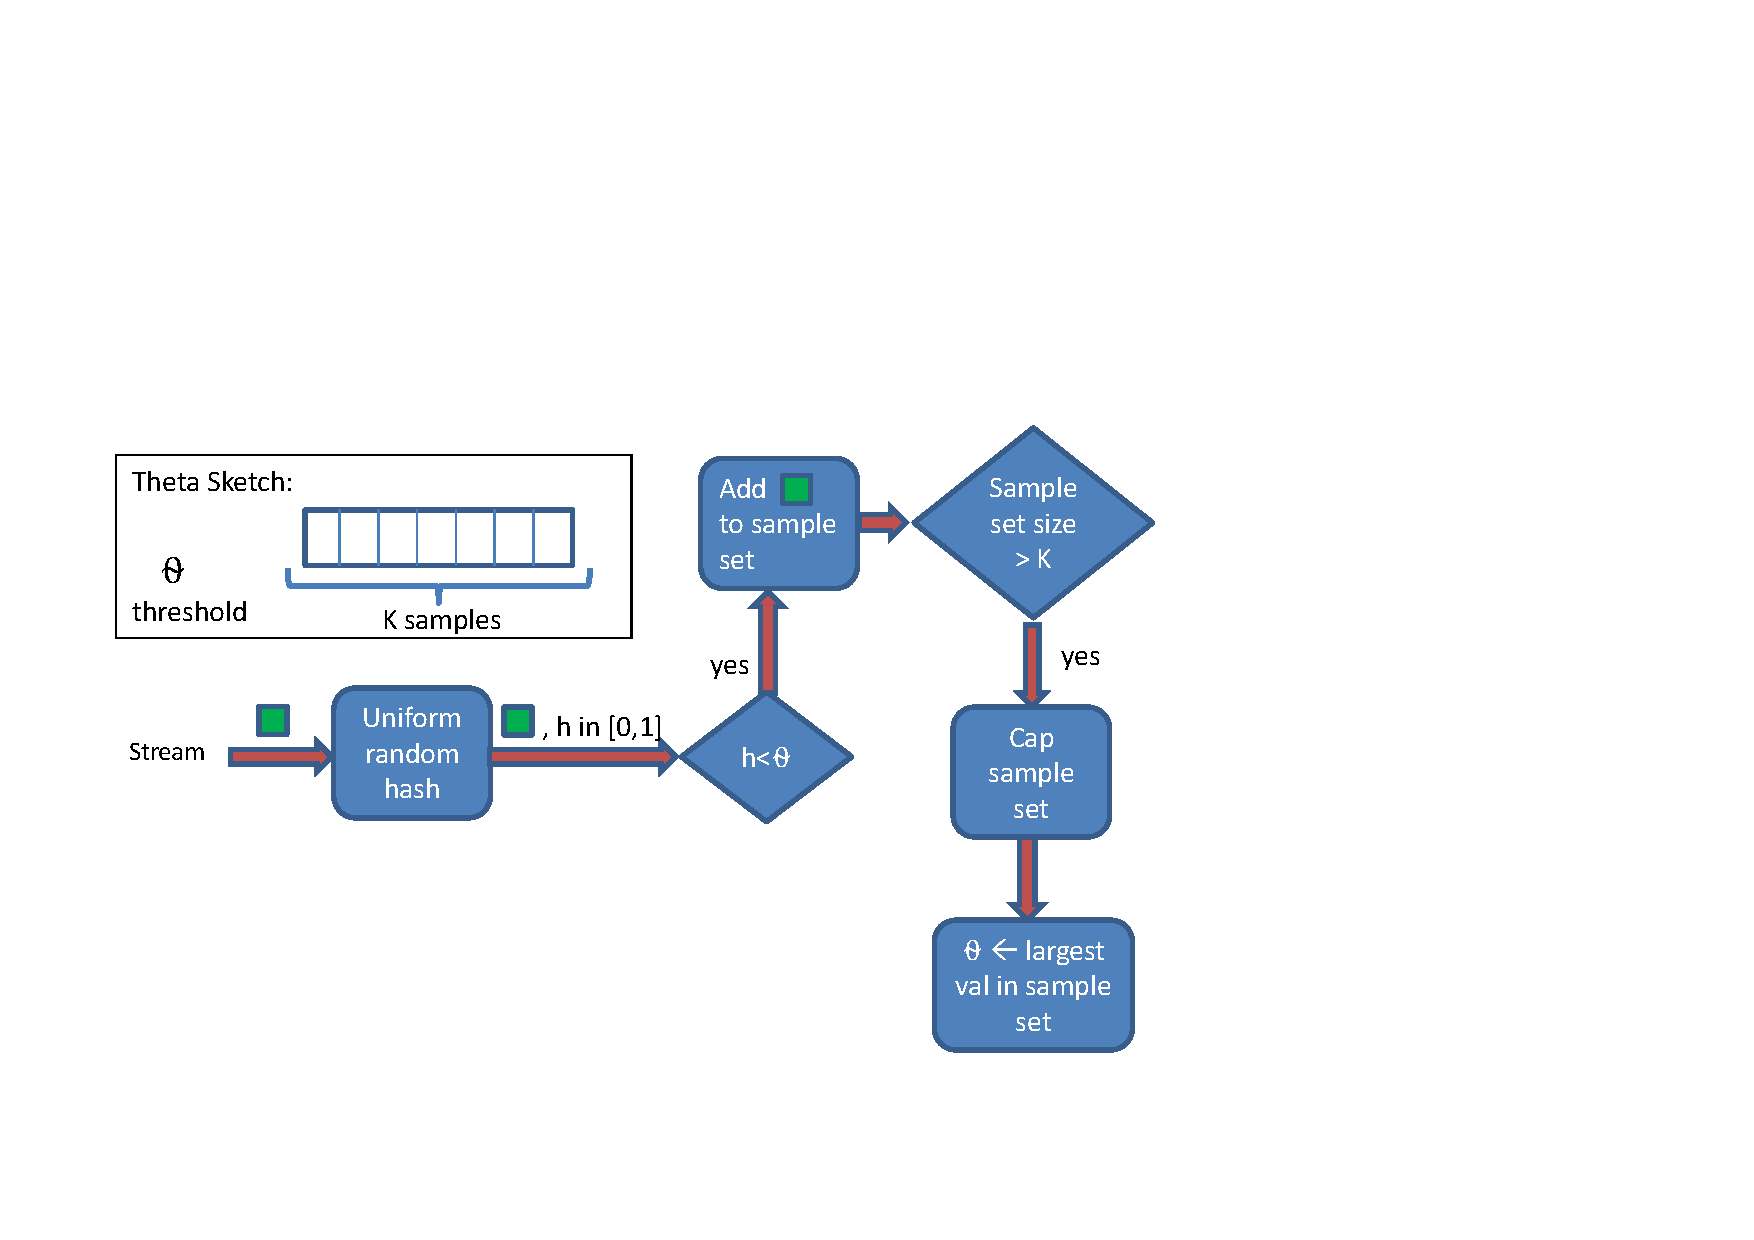
\includegraphics[width=3.5in]{images/seqTheta.pdf}
    \caption{Theta sketch algorithm.}
    \label{fig:thetaSampling}
\end{figure}





\subsection{Concurrent Algorithm}
\label{ssec:concurrent-theta}

%As mentioned in Section~\ref{sub:concurency}, 
Our concurrent implementation -- given in  Algorithm~\ref{alg:concurrent-theta} 
and illustrated in Figure~\ref{fig:concurrentTheta} --  
uses multiple threads to process incoming stream elements; 
it services queries at any time during the sketch's construction. 
%Since the only thing threads need to know in order to sample stream elements is
%the value of $\Theta$, they can do so locally in parallel, 
Update threads sample stream elements in parallel into local buffers, 
while a background thread periodically propagates the sampled values to a shared sketch
consisting of sampleSet and $\Theta$. 


\begin{algorithm*}[tb]
\small
\begin{multicols}{2}
\begin{algorithmic}[1]

%\State {\bf Sketch variables:}
\Vars
\State   sampleSet, init $\emptyset$ \Comment global samples
\State  $\Theta$, init $1$			\Comment global threshold
\State {\tt atomic} est, init $0$ \Comment estimated \# uniques
\State $h$, init random uniform hash function 
\Statex
\ForEach{update thread $t_i$} 
	\State \emph{buf$_i$}, init $\emptyset$ \Comment local sample set
	\State \emph{aux$_i$}, init $[ ]$ \Comment auxiliary array
	\State $\Theta_i$, init $1$ 	\Comment local threshold
	\State {\tt atomic} $P_i$, init $1$ \Comment for synchronization
\EndFor
\EndFor

\Statex
\Procedure{query}{}
\State return est \label{l:query}
\EndProcedure
%\Statex

\Procedure{update$_i$}{val}
\If{$h$(val) $< \Theta_i$} 
	add val to \emph{buf$_i$} \label{l:local-sample}
\EndIf
\If{$|$\emph{buf$_i$}$| > b$} \Comment propagate
	\State wait until $P_i >0$ \label{l:wait}
	\State $\Theta_i \leftarrow P_i$ \label{l:adopt}
	\State \emph{aux$_i$}  $\leftarrow$ sort by $h$ $\{ e \in \mathit{buf_i} | h(e) <\Theta_i \}$
		\label{l:sort}
	\State $P_i \leftarrow 0$ 		\label{l:signal}
	\State \emph{buf$_i$}$ \leftarrow \emptyset$  \label{l:clean} 

\EndIf  
\EndProcedure

\Procedure{propagator}{}
\While {true}
\ForAll{update thread $t_i$ s.t. $P_i =0$} 
		\State  update sampleSet and $\Theta$ with \emph{aux$_i$} \label{l:aux}
		\State est $\leftarrow |$sampleSet$|/ \Theta$ \label{l:update-est}
		\State $P_i \leftarrow \Theta$  \label{l:theta}
\EndFor
\EndWhile
\EndProcedure

\end{algorithmic}
\end{multicols}
\caption{Concurrent $\Theta$ sketch algorithm.}
\label{alg:concurrent-theta}
\end{algorithm*}

The key to achieving efficiency is exploiting locality and minimizing synchronization.
Every worker thread $t_i$ samples stream elements into a local bounded buffer 
\emph{buf$_i$} of size $b$ (line~\ref{l:local-sample}). 
To avoid frequent cache invalidations, $t_i$ uses a periodically refreshed
local copy $\Theta_i$ of $\Theta$. 
Because the global  $\Theta$ is monotonically decreasing, periodically copying it
into local copies maintains the invariant $\Theta_i \geq \Theta$.
Thus, while threads may over-sample, they never fail to sample elements that need 
to be included in the shared sketch. 
%Initially, all buffers are empty and all local $\Theta_i$s are $1$. 

When the buffer of a thread $t_1$ becomes full, $t_1$ sorts it
into an auxiliary array \emph{aux$_i$} and signals to the propagator  to merge
it with the shared sketch (lines~\ref{l:sort}--\ref{l:signal}).
In the meantime, $t_1$ proceeds to re-fill its buffer with new samples.
The propagation  (line~\ref{l:aux}), in turn,  is highly optimized, as it merges a sorted array of 
values into the sampleSet, and can stop merging upon encountering 
an element whose hash is bigger than the global $\Theta$.

Update thread $t_i$ synchronizes with the propagator using a 
single \emph{atomic} variable $P_i$, which it sets to zero 
to signal to the propagator that the auxiliary array is ready.  
Because $P_i$ is  atomic, the Java memory model
guarantees that $t_i$'s auxiliary array is visible to
the background thread when $P_i$'s update is.
This is  an expensive operation (involving a memory fence),  
but we do it only once per $b$ items retained in the sample.

Before propagating its buffer, $t_i$ waits
until $P_i > 0$  (line~\ref{l:wait}); 
this indicates that the propagation of the previous \emph{aux}$_i$
 has completed, and  \emph{aux}$_i$ may
be reused. Thus, we  ensure that the sketch uses bounded space.
%
When the background thread completes the propagation, 
it piggybacks the global $\Theta$, which only it updates, on $P_i$  (line~\ref{l:theta}), 
and $t_i$ adopts it  (line~\ref{l:adopt}). Thus, update threads   learn $\Theta$ at no
additional synchronization cost. 

In order to support  fast concurrent reads, the shared sketch
maintains an atomic variable est, estimating the number of
 unique items seen so far by the propagator.
The background thread updates this variable after each propagation.
Again, because est is atomic, updating it involves a costly memory fence, which we amortize by performing it once per $b$ updates. 

For the $S$.union($S'$) operation (omitted from the code), 
we assume $S'$ is not undergoing any updates. 
The propagator thread puts its normal tasks on hold, 
 adopts the smaller $\Theta$ of the two sketches, merges their sampleSets while filtering elements according to the new $\Theta$, updates est, and resumes its 
 propagation tasks. Other operations (query and update) continue undisturbed.


\begin{figure}[tb]
%    \centering
    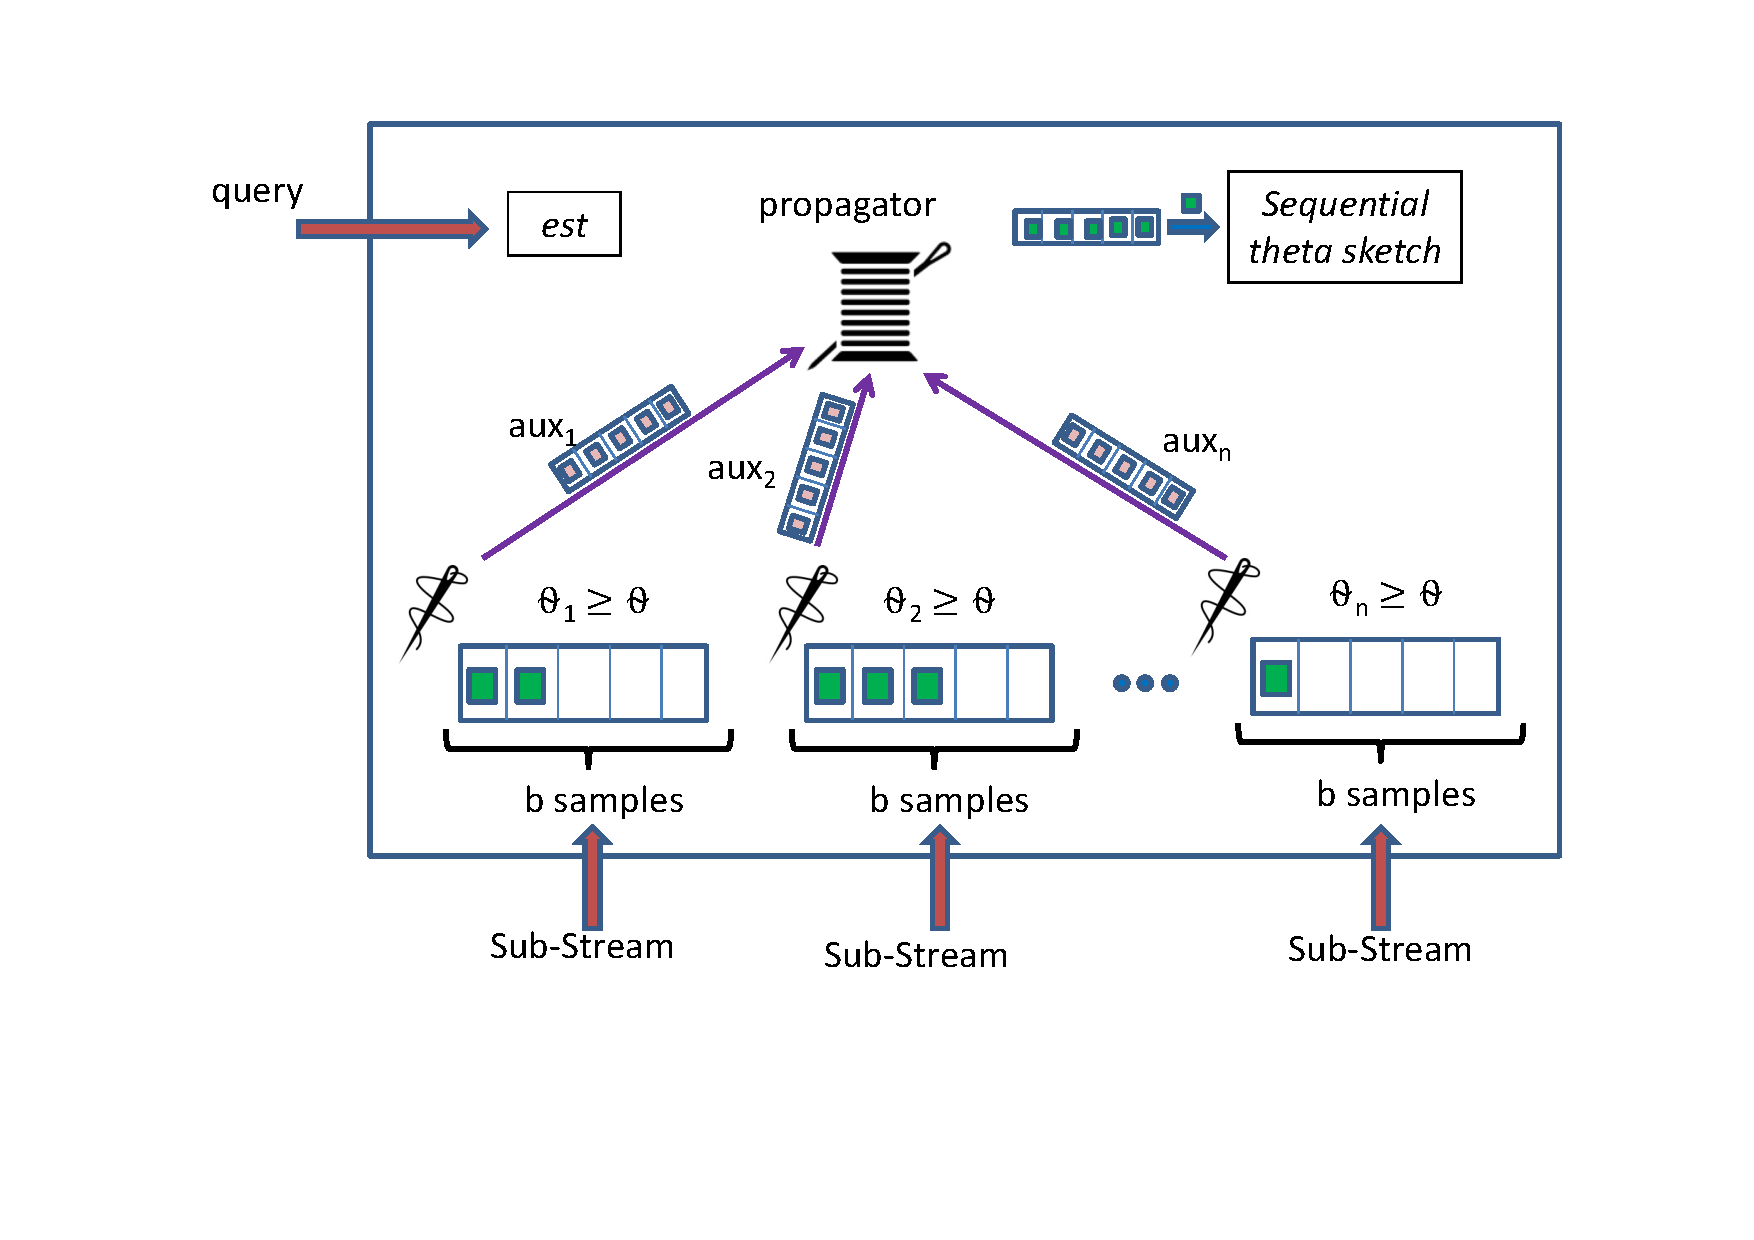
\includegraphics[width=3.5in]{images/concTheta.pdf}
    \caption{Concurrent $\Theta$ sketch architecture.}
    \label{fig:concurrentTheta}
\end{figure}
